④ つぎの伝達関数のゲイン線図(ボード線図のゲインの図)を,折れ線近似を用いて描け.ただし,折れ
点の周波数とそのときのゲインのデシベル値がわかるように描くこと.
$$
\frac{10(s+10)}{s(s+1)(s+100)}
$$


$$
\frac{10(s+10)}{s(s+1)(s+100)}=\frac{10 \cdot 10(0.1 s+1)}{100 s(s+1)(0.01 s+1)}= \frac{1}{s} \cdot \frac{1}{s+1} \cdot \frac{1}{0.01 s+1} \cdot(0.1 s+1)
$$
\begin{figure}[H]
    \centering
    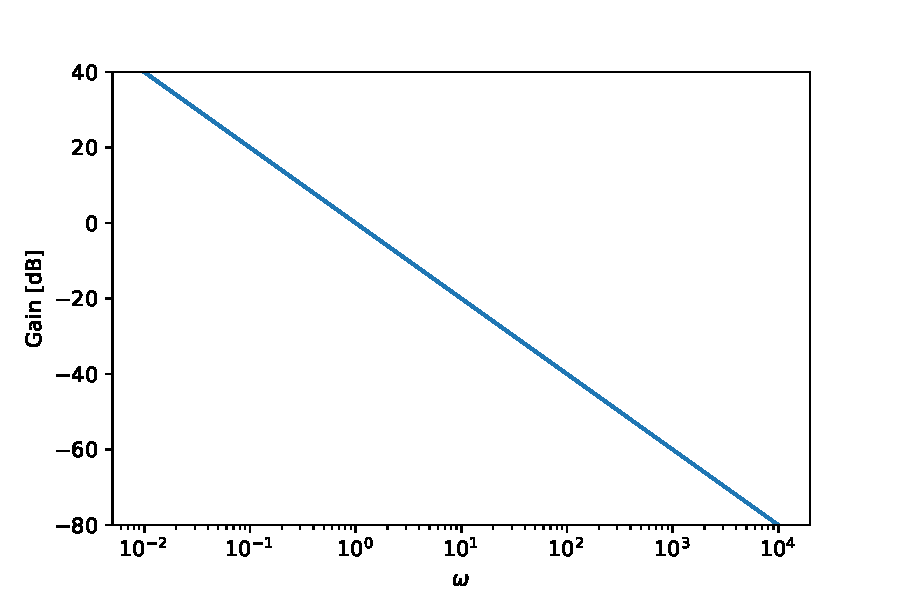
\includegraphics[scale=0.75]{1.pdf}
    \caption{$\frac{1}{s}$のゲイン曲線}
\end{figure}
\begin{figure}[H]
    \centering
    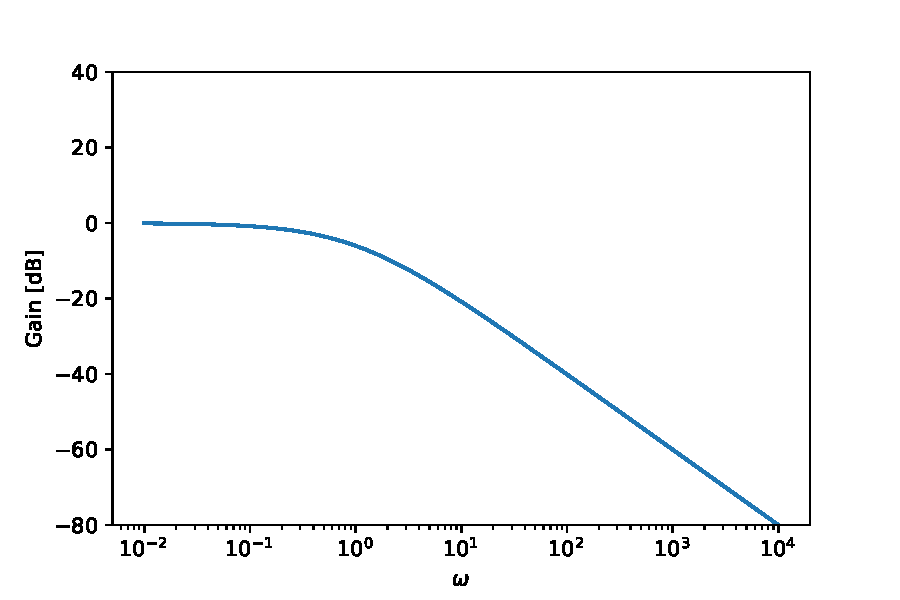
\includegraphics[scale=0.75]{2.pdf}
    \caption{$\frac{1}{s+1}$のゲイン曲線}
\end{figure}
\begin{figure}[H]
    \centering
    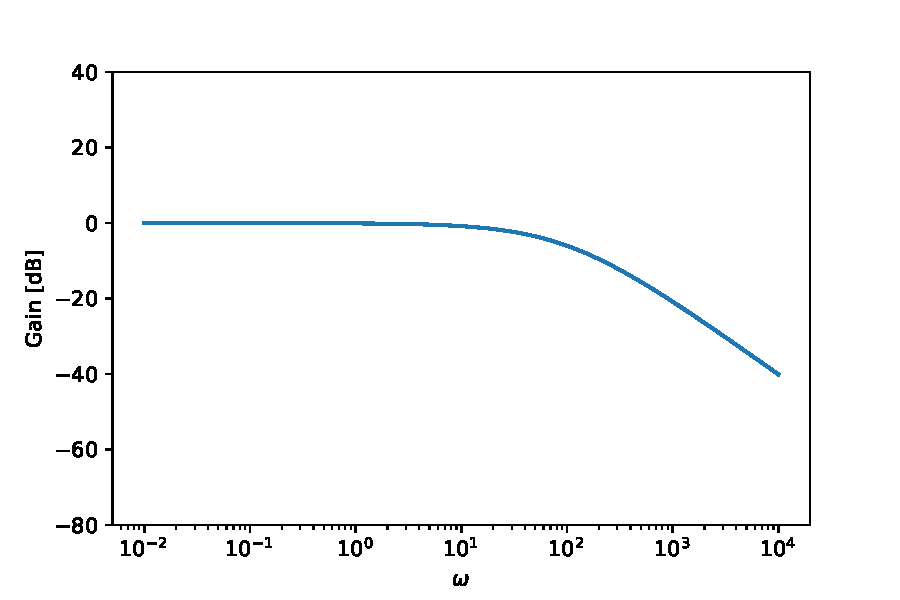
\includegraphics[scale=0.75]{3.pdf}
    \caption{$\frac{1}{0.01s+1}$のゲイン曲線}
\end{figure}
\begin{figure}[H]
    \centering
    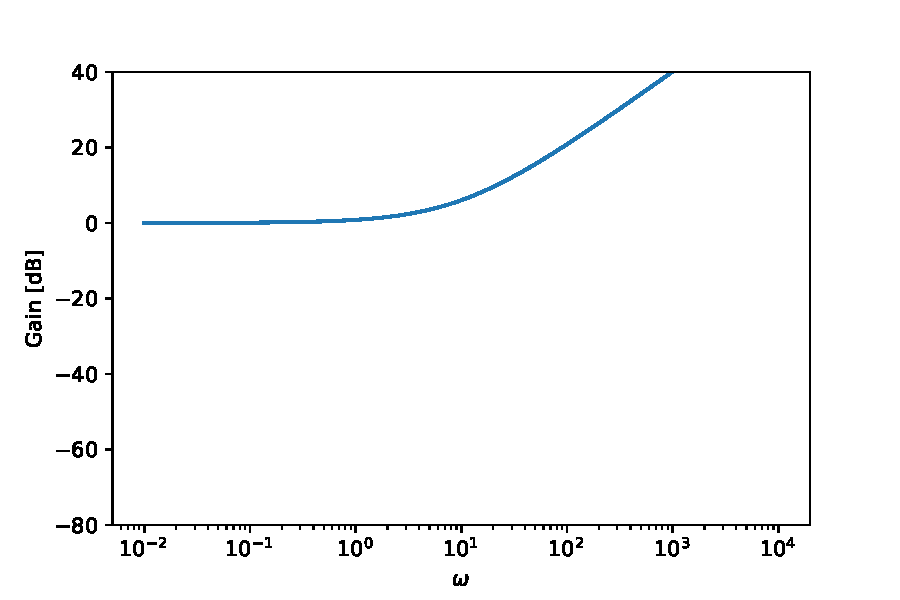
\includegraphics[scale=0.75]{4.pdf}
    \caption{$0.1s+1$のゲイン曲線}
\end{figure}
\begin{figure}[H]
    \centering
    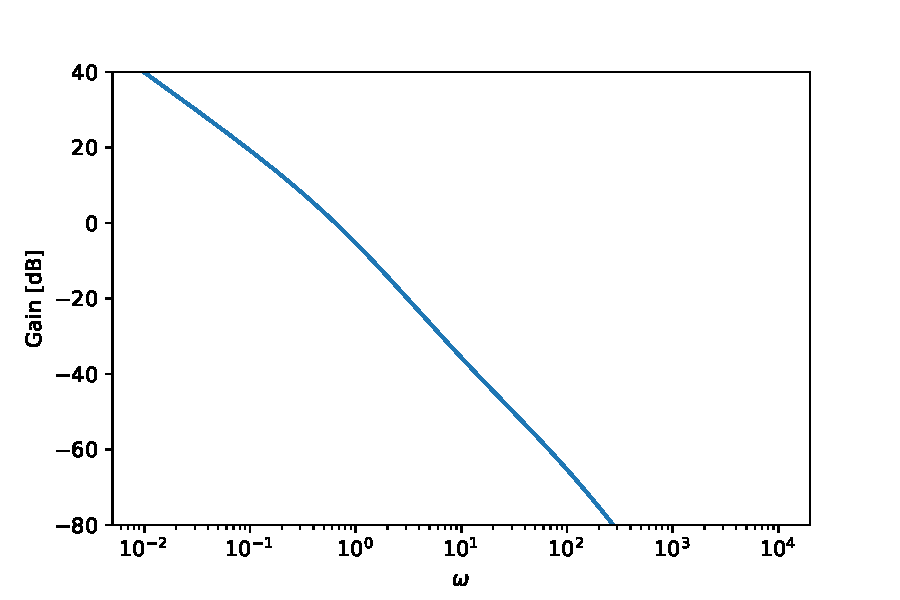
\includegraphics[scale=0.75]{5.pdf}
    \caption{与えられた伝達関数のゲイン曲線}
\end{figure}

\newpage
